By looking at the polarization morphology, made uup of polarization vectors, we can infer the dominant polarization mechanisms within the disk, and by doing this at each band, we can see how the morphology changes. We start by getting the polarization vectors, and then later we will create models to fit the morphologies. 



A vector could be made at each \add{how we make each vector}.


\textbf{Sampling:} The Nyquist-Shannon sampling theorem was used to determine the pixel spacing between vectors to make sure we are not under- or over-sampling relative to the size of the beam at each band. 

To follow this sampling, we ensure that the distance between each vector is no larger than half of the size of the beam. To do this, we take the size of the beam in pixels by:
\begin{equation}
    \text{Beam Size =} \sqrt{BMAJ \cdot BMIN},
\end{equation}
\noindent where $BMAJ$ and $BMIN$ are the sizes of the major and minor axes of the beam in units of pixels. Then the sampling step is taken to be the the nearest integer of Beam Size/2. The steps between each vector for each band are summarized in Table \ref{tab: vector_info}. 


\textbf{Vector Length:} The length of these vectors are all normalized to the same length, and are not scaled based on the strength of the (\SI or \POLIsym) value at its corresponding pixel. The length of these vectors were chosen using guess and check, and just scaled to what looks best. The length of the vectors for each band are summarized in Table \ref{tab: vector_info}. 

\textbf{Testing Reliability:} Beyond the step size, we also have to ensure that the vector is reliable. The vector is plotted if it meets the conditions:
\begin{equation}
    \frac{\POLIeq}{\POLIerreq} >  \quad \text{ and } \PAerr < 10^\circ,
    \label{eq: vector_conditions}
\end{equation}
\noindent where $\sigma_\theta$ is the uncertainty for polarization angle in degrees. These conditions were chosen based on the ones from \cite{sadavoy_dust_2019}, without the condition that $I/\sigma_I>3$ since IRS 63 is so bright and well-resolved, this condition was not necessary for our analysis. 




\begin{table}[h!]
\centering
\caption{\add{caption}}
\begin{tabular}{ccccccc}
\toprule
\multirow{2}{*}{} & \multicolumn{3}{c}{\textbf{Stokes Errors (mJy)}} & \textbf{Step} & \textbf{Vector Length} &  \\
& I & Q & U & pix  &  pix & \\
\midrule 
\textbf{Band 4} & Ierr & Qerr & Uerr & 4 & 2 \\
\textbf{Band 5} & 0.0143745 & 0.013025 & 0.01525  & 8 & 6   \\
\textbf{Band 6} & Ierr & Qerr & Uerr & 6 & 4   \\
\textbf{Band 7} & 0.035175 & 0.02625 & 6 & 6 & 4 \\
\bottomrule
\end{tabular}
\label{tab: vector_info}
\end{table}

















\begin{figure*}[h]
  \centering
  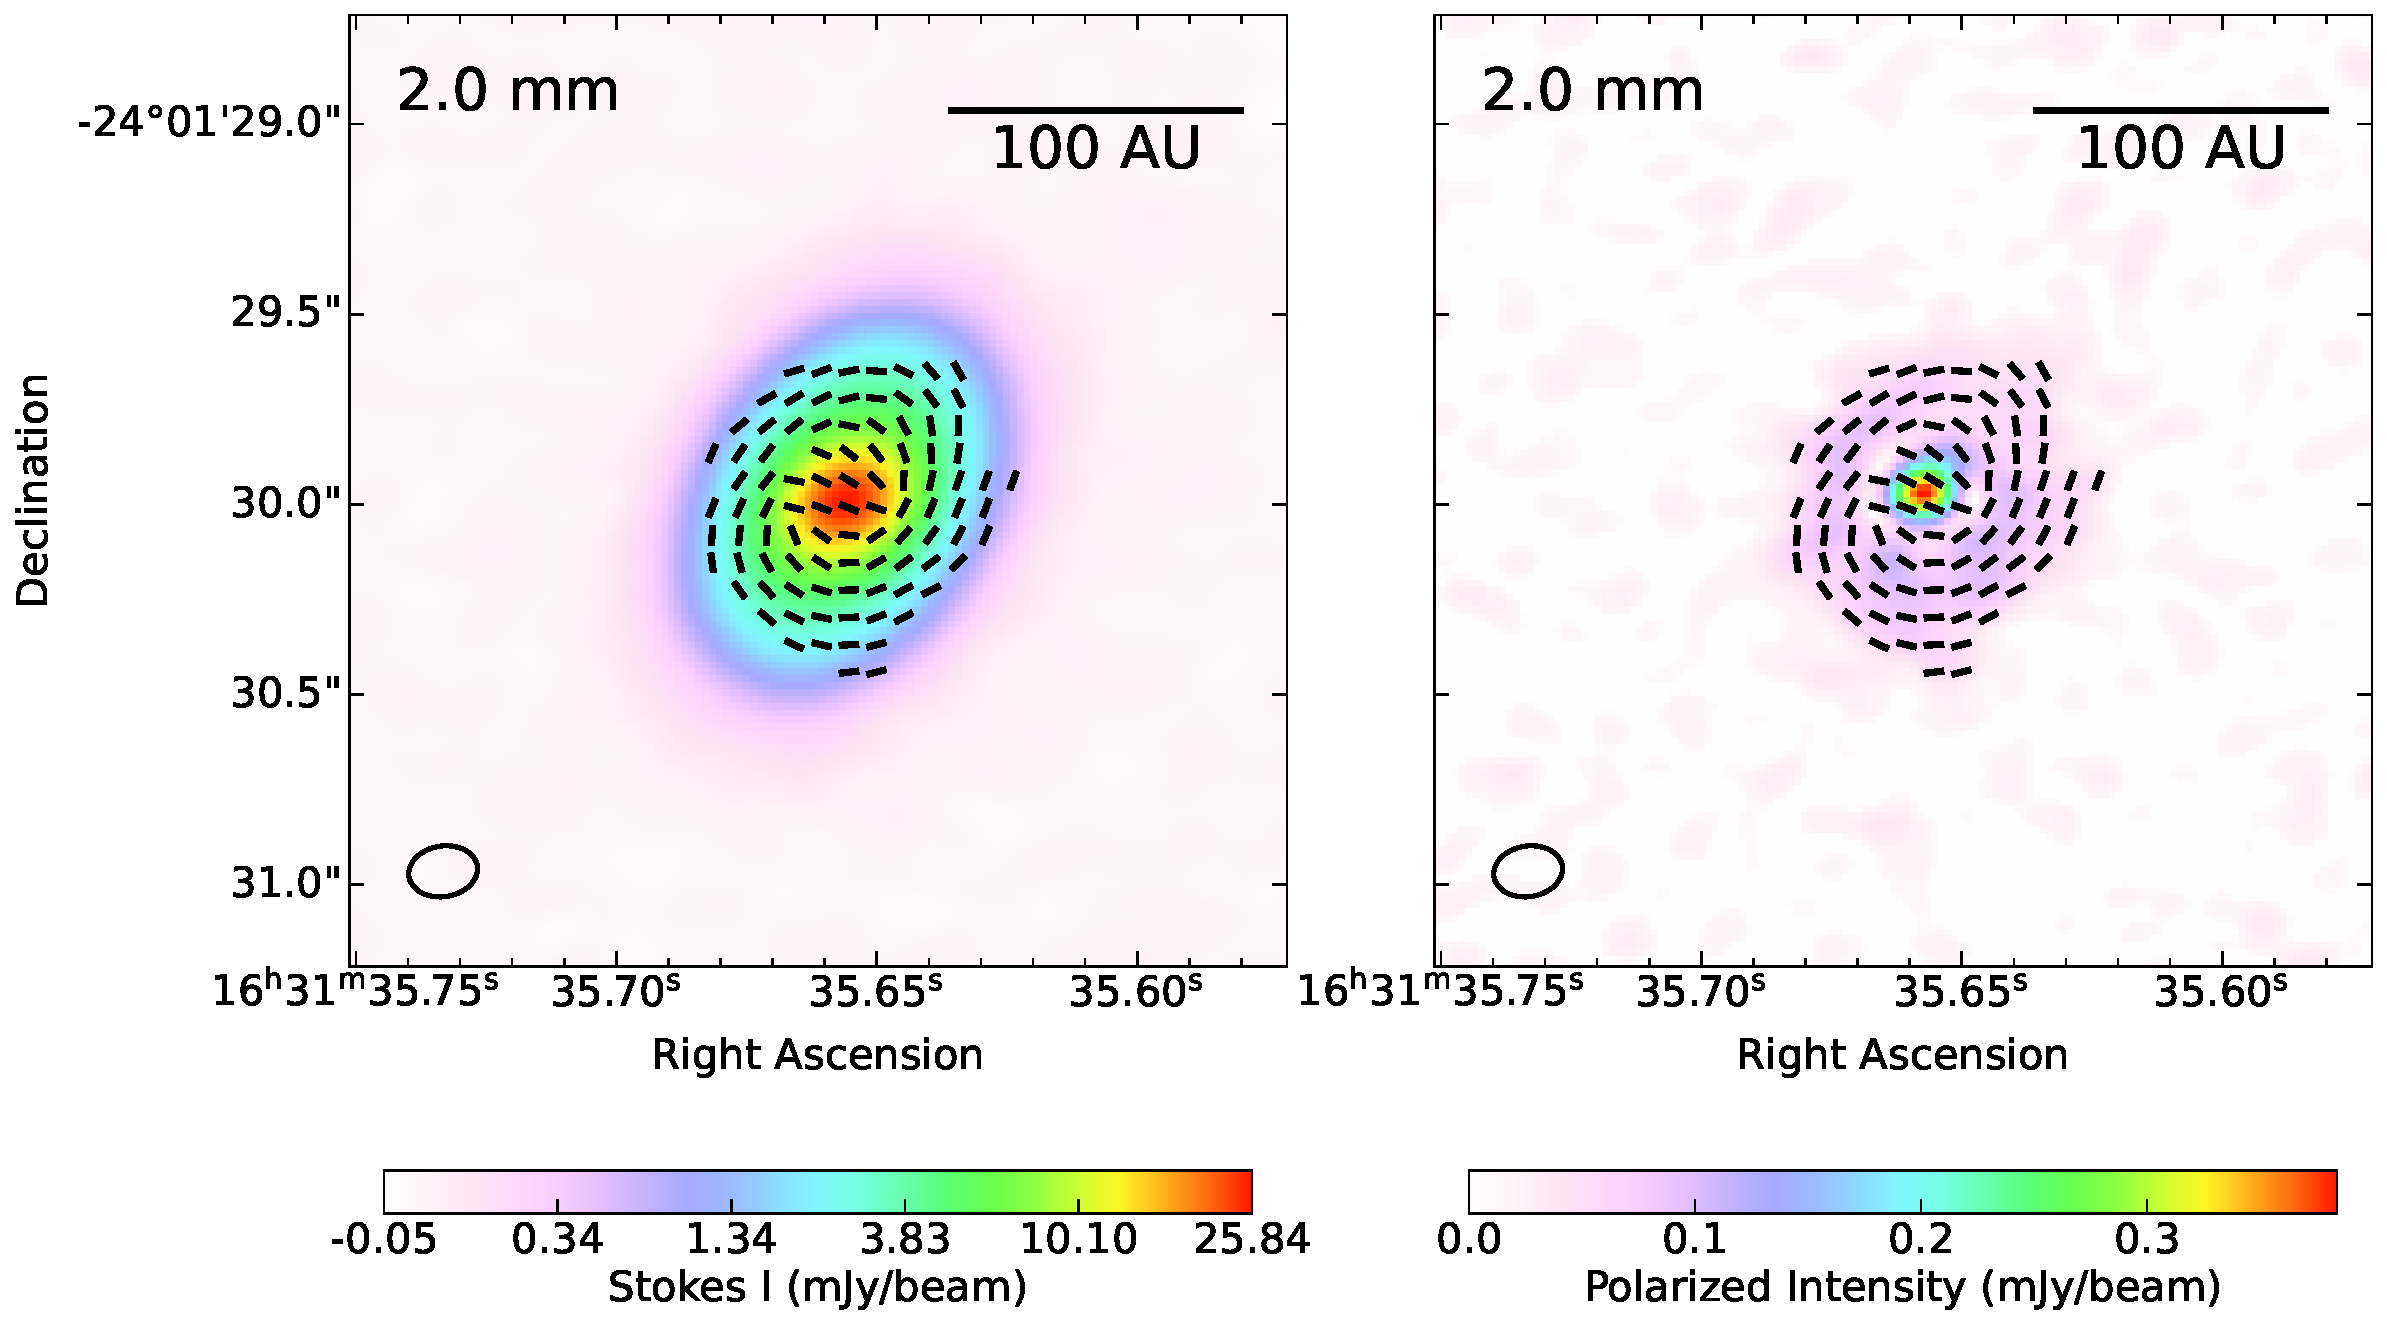
\includegraphics[width=1.1\textwidth]{WRITEUP_AND_IMAGES/IMAGES/WRITEUP/StokesI_POLI/IRS63_StokesI_POLI_vectors_BAND4.pdf}
  \caption{\quoted{\stokesI (left) and polarized intensity (right) for IRS 63 at ALMA Band 4 (\bandfourlambda). The polarization vectors are shown as black lines. Vectors are shown for pixels with \add{conditions}. The beam is shown in the lower left corner. The \stokesI maps have a log colour scale and the polarized intensity maps have a linear scale \cite{sadavoy_dust_2019}}}
  \label{fig: StokesI_POLI_B4}
\end{figure*}


\begin{figure*}[h]
  \centering
  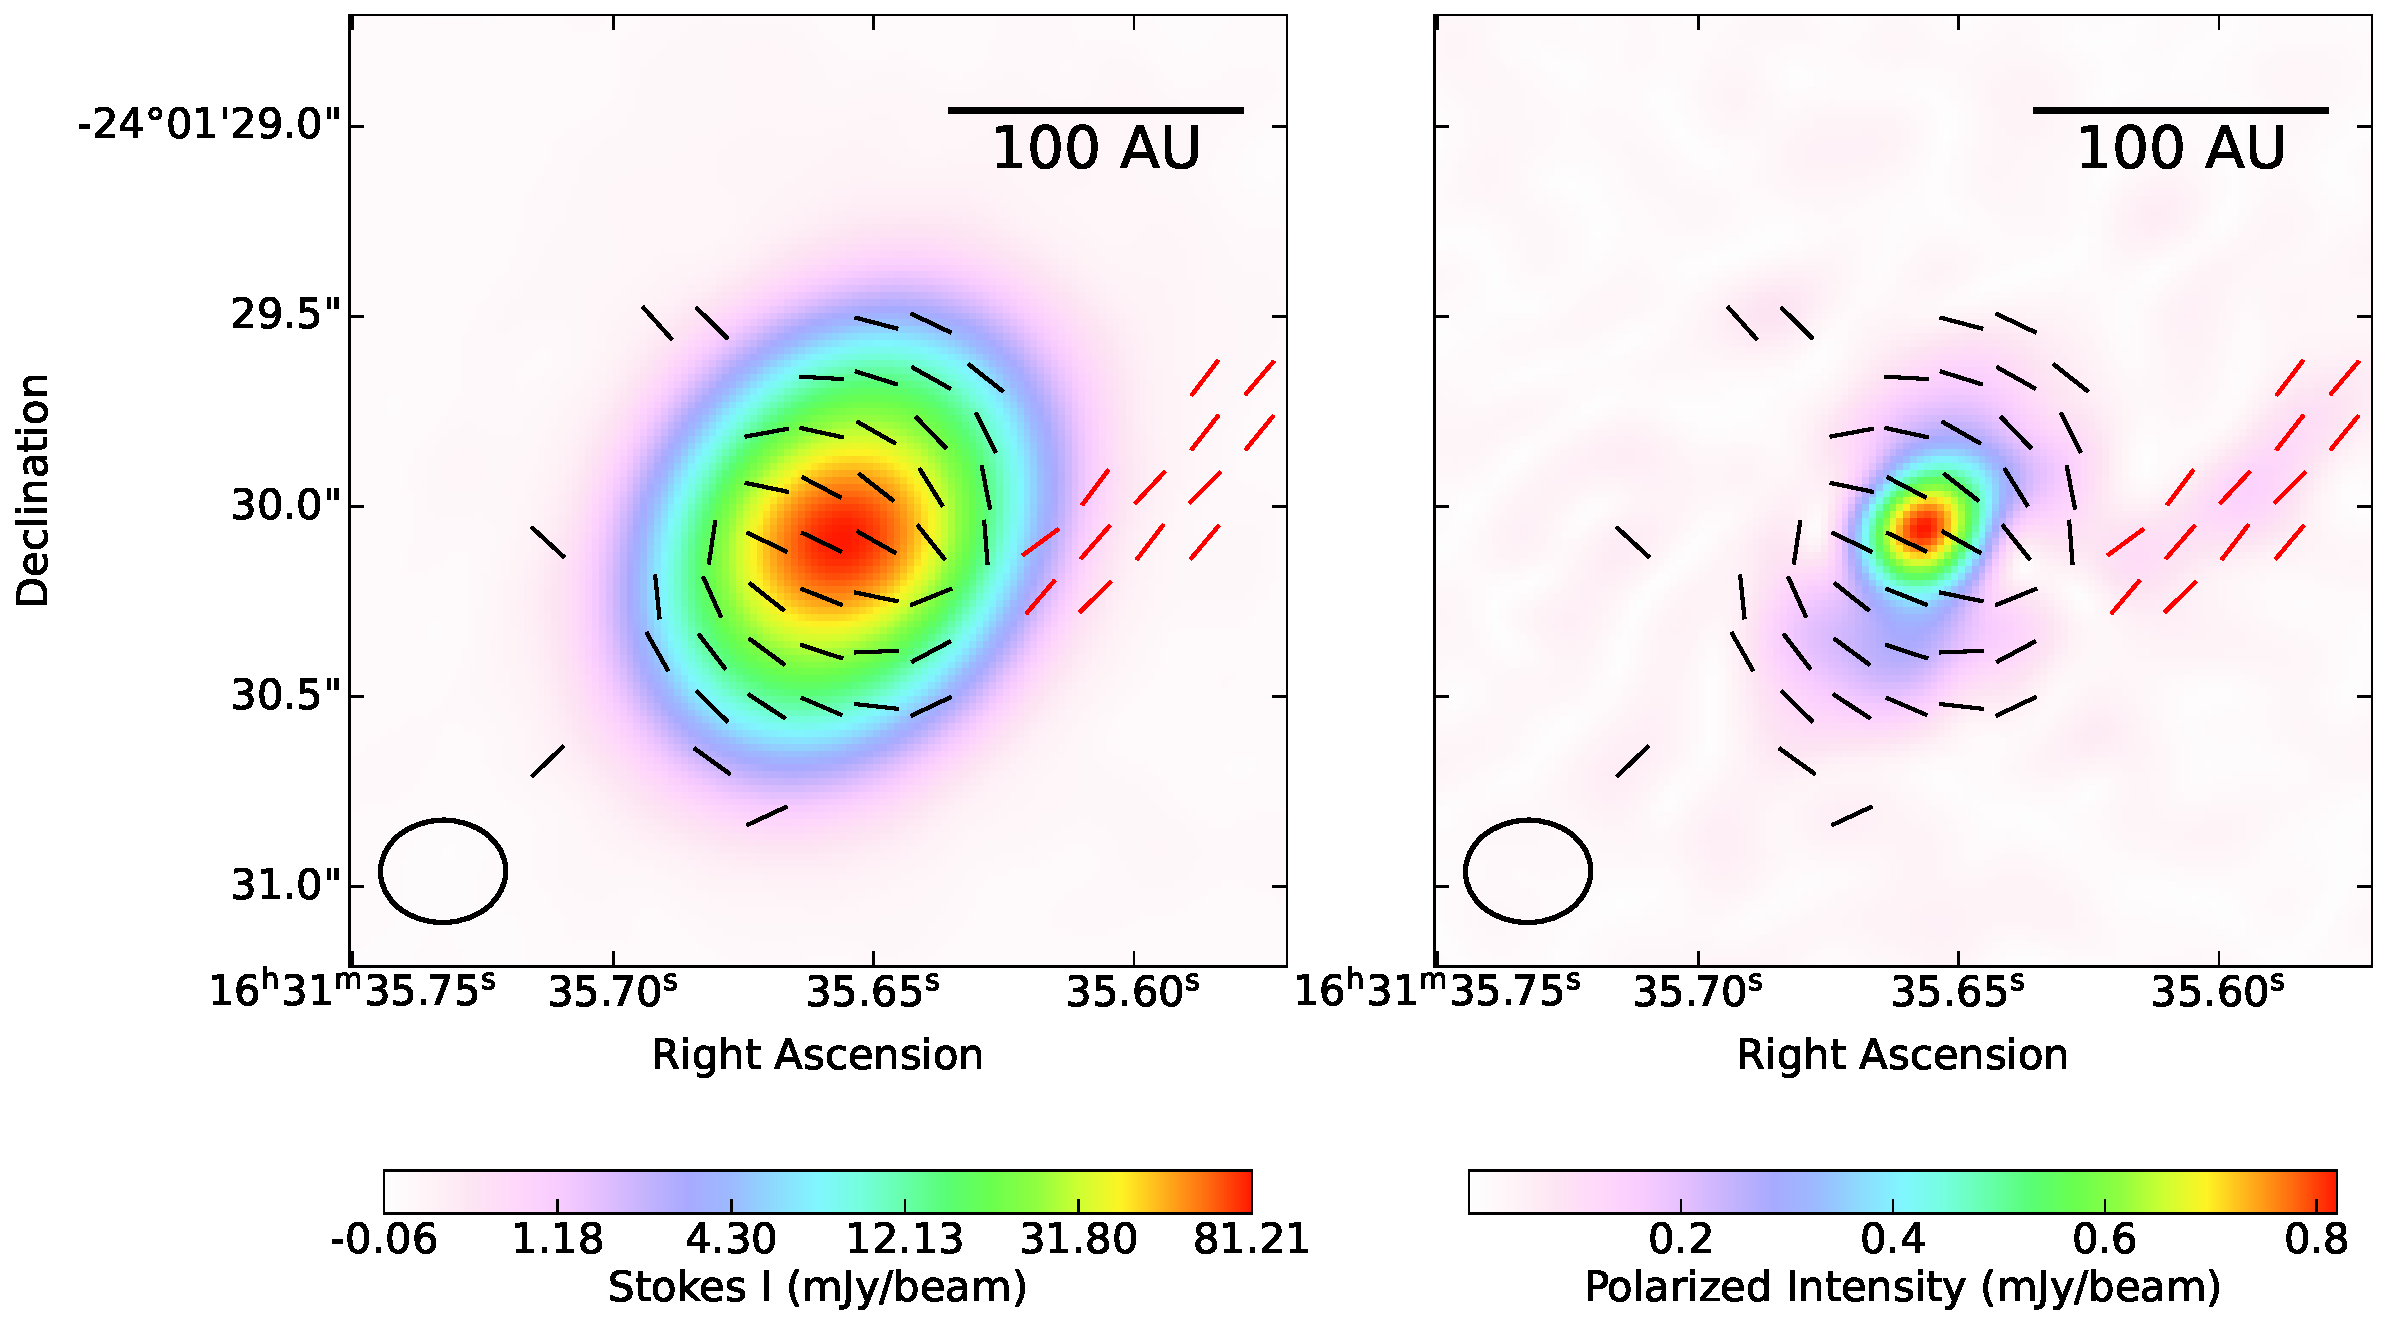
\includegraphics[width=1.1\textwidth]{WRITEUP_AND_IMAGES/IMAGES/WRITEUP/StokesI_POLI/IRS63_StokesI_POLI_vectors_BAND5.pdf}
  \caption{Same as Figure \ref{fig: StokesI_POLI_B4}, except for Band 5 (\bandfivelambda).}
  \label{fig: StokesI_POLI_B5}
\end{figure*}



\begin{figure*}[h]
  \centering
  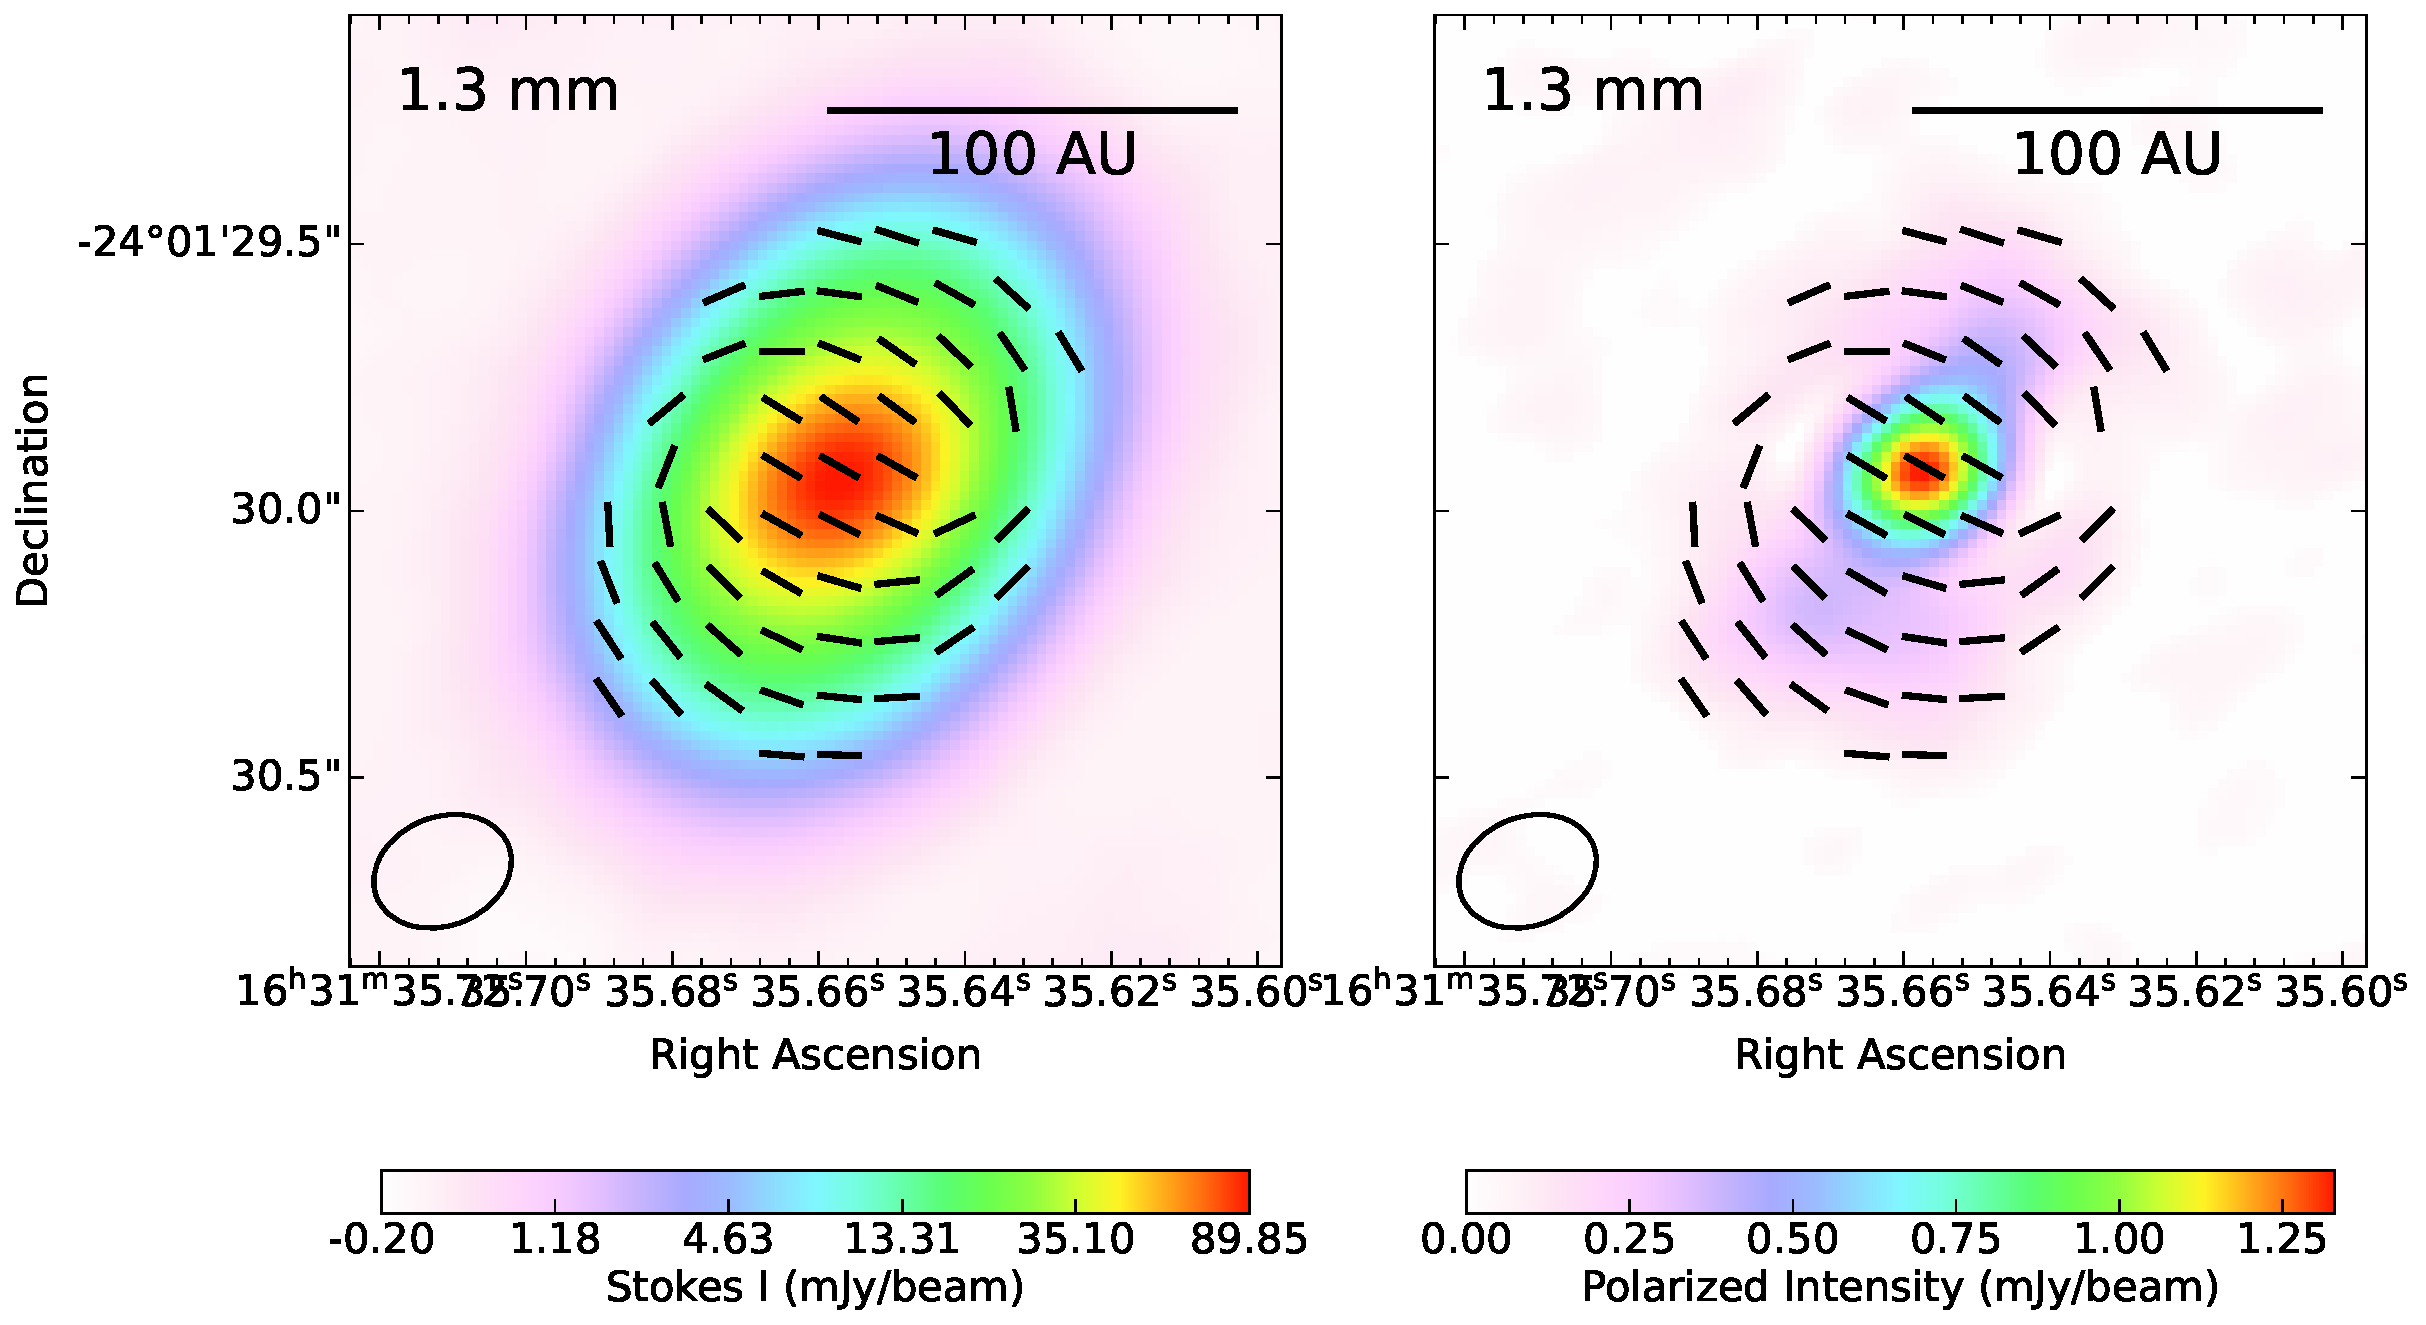
\includegraphics[width=1.1\textwidth]{WRITEUP_AND_IMAGES/IMAGES/WRITEUP/StokesI_POLI/IRS63_StokesI_POLI_vectors_BAND6.pdf}
  \caption{Same as Figure \ref{fig: StokesI_POLI_B4}, except for Band 6 (\bandsixlambda).}
  \label{fig: StokesI_POLI_B6}
\end{figure*}


\begin{figure*}[h]
  \centering
  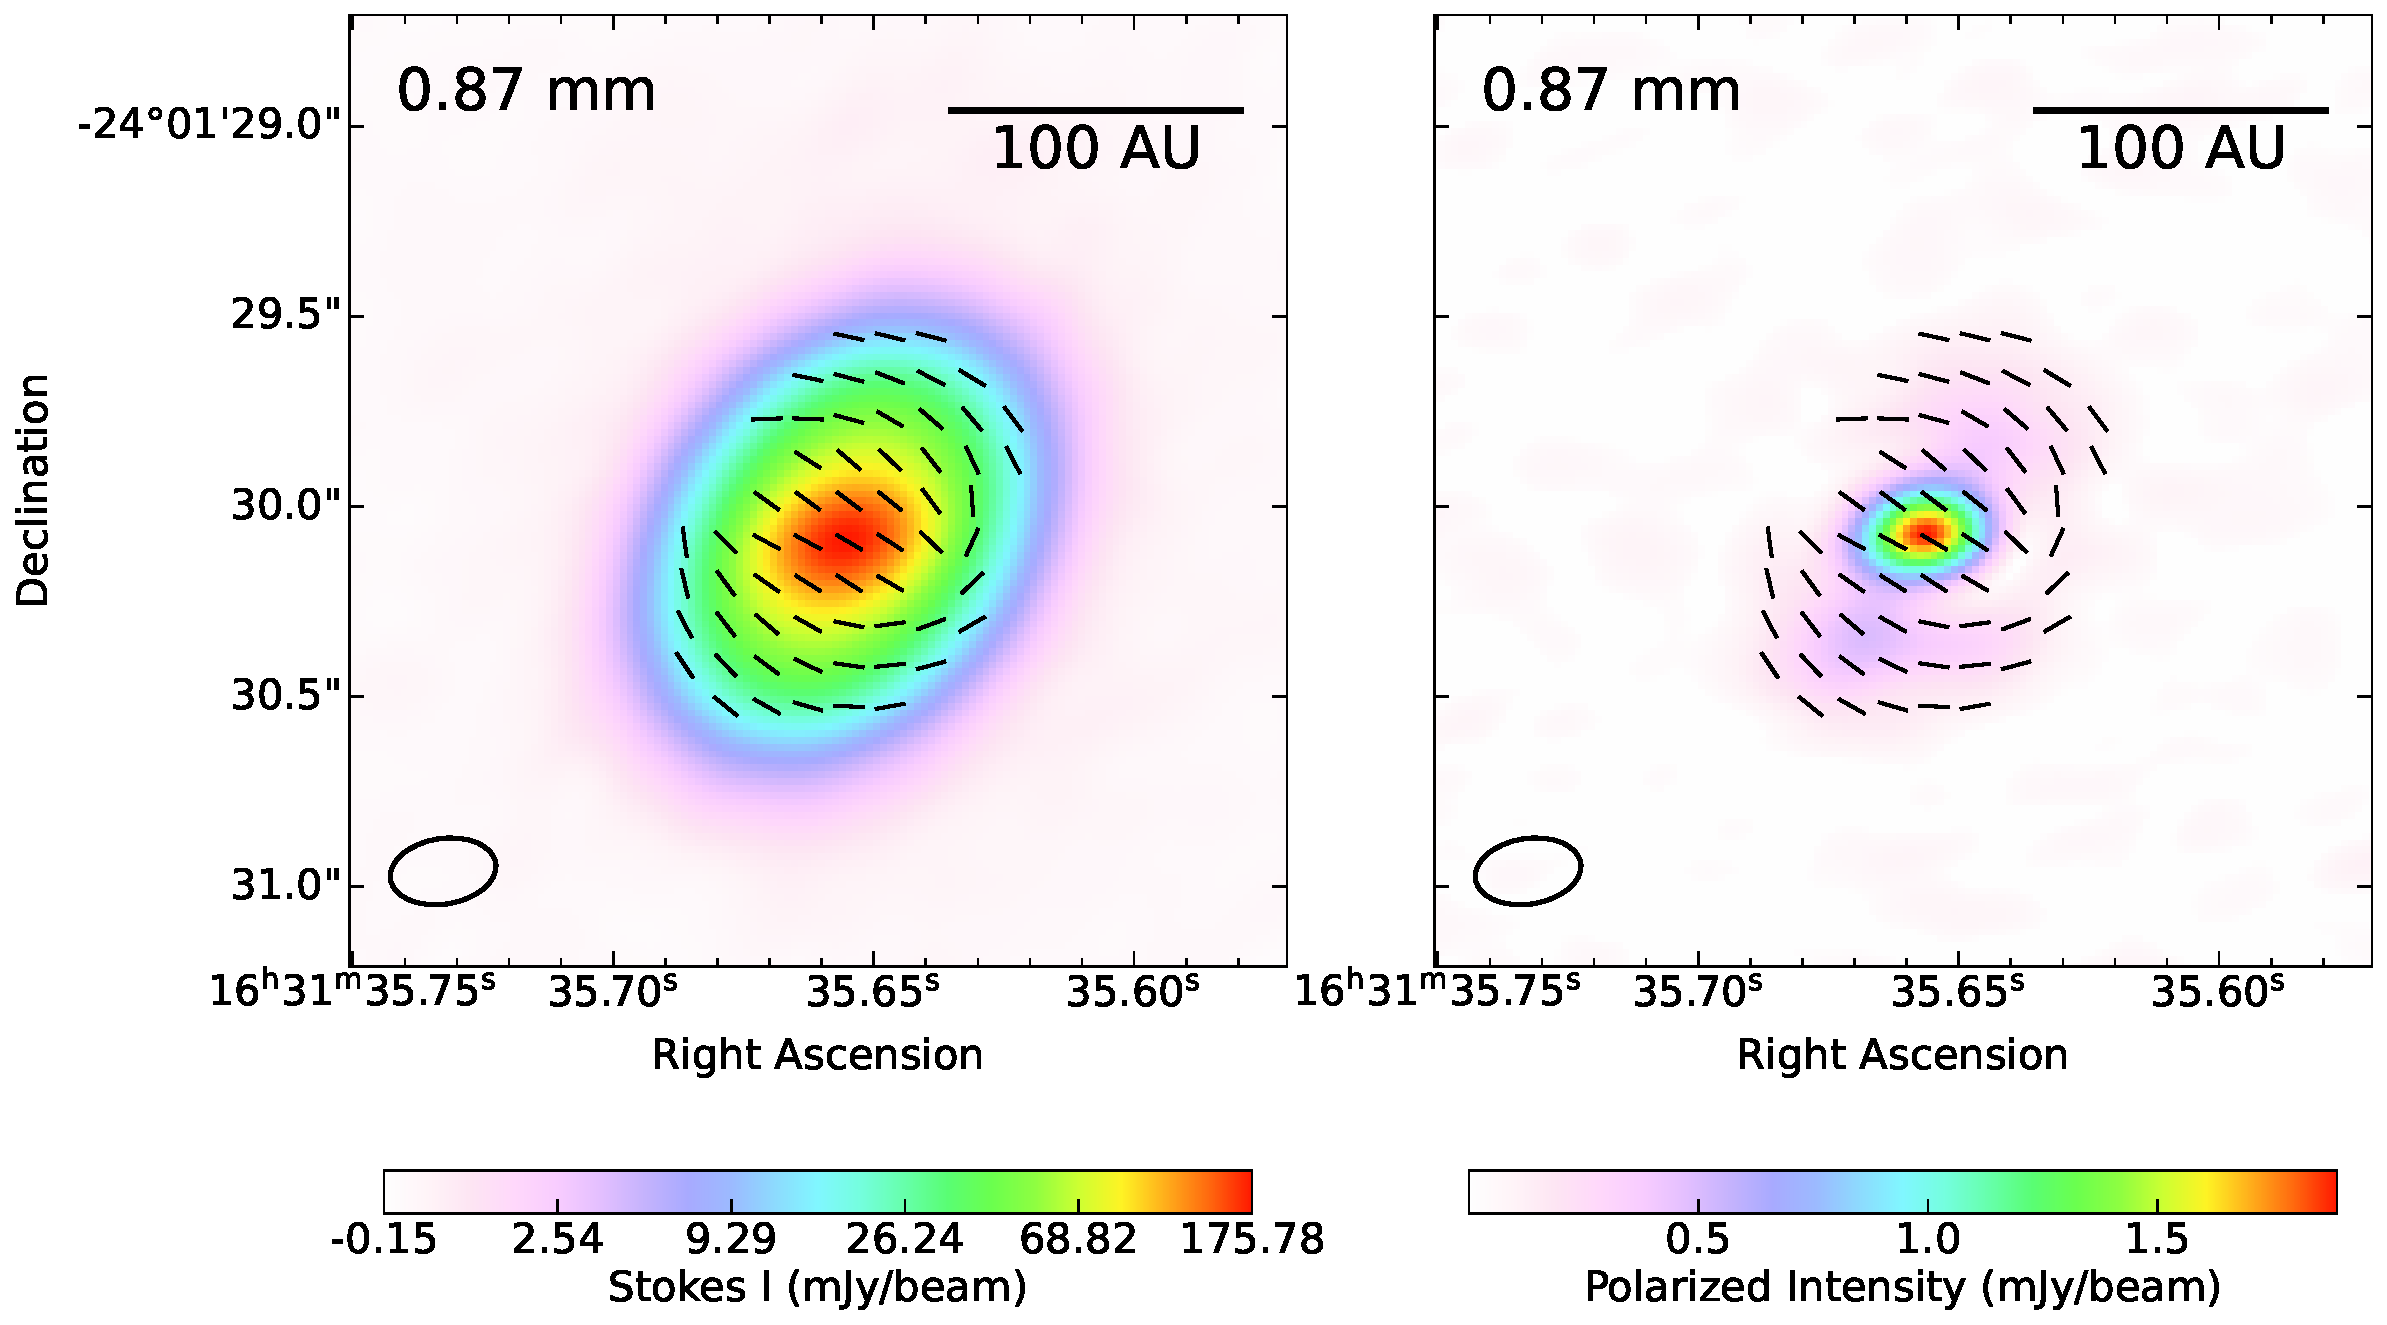
\includegraphics[width=1.1\textwidth]{WRITEUP_AND_IMAGES/IMAGES/WRITEUP/StokesI_POLI/IRS63_StokesI_POLI_vectors_debiased_BAND7.pdf}
  \caption{Same as Figure \ref{fig: StokesI_POLI_B4}, except for Band 7 (\bandsevenlambda).}
  \label{fig: StokesI_POLI_B7}
\end{figure*}


